\section{Summary}
If we evaluate any product, it would certainly have some pros and cons. No product is full of faults and no product is perfect.Same is the case with the case, as it is targeting a specific group so it has a diverse kind of effect. 
\subsection{Positives}
If we talk about positives in Embold, we can easily say it is focusing on user needs i.e
\begin{itemize}
\item It has a lot of options which can be helpful for all the user groups. It gives a detail about code design, hotspot issues, duality, which is equally helpful for every stake holder. 
\item It has very diverse package plans for enterprises, SMEs and startups. Also it is helpful for onetime user or someone who does not have many repositories to test. Also the price plans are very much affordable. 
\item Problem which was targeted is well addressed and it gives quite extra-ordinary results. As it gives in dept view about various aspects.
\item Outstanding Contact section, on-line chat, on call and email option.
\item On premise, cloud availability makes it a very usable and portable application, it defines the quality. 
\item Compatibility with different version control systems i.e GItLab, BitBucket,GitHub.
\end{itemize}
\subsection{Negatives}
There are also few negatives i.e
\begin{itemize}
\item The UI is not very aesthetic it looks very unattractive. No proper and significant hovering while navigating through the web, especially in the navigation bar.
\item  Lack of colour variety, and too much text. The size of the text is not eye catching. 
\item Not very dynamic web design, looks quite static website. 
\item Time on Task was pretty high, as most of the time it took a long to search and navigate. 

\end{itemize}
\section{Recommendation for Improvements}
There can be lot of improvements in the Embold by a variety of ways; 
\begin{itemize} 
\item The website is not very efficient. It can be improved.
\item  As we can see in Figure \ref{fig:improve} that there is a room to add more programming languages.
\item The time which it took for scanning can be improve. 
\item Availability in dark mode could be a nice add-on.
\item Different Colour schemes can be applied or the better UI and also more significance to signifiers and identifiers by applying some better hovering methods could be a considerable gain.
\item Better documentation and less text on the main page could attract more users.   
\end{itemize}
\begin{figure}[htbp]
\begin{center}
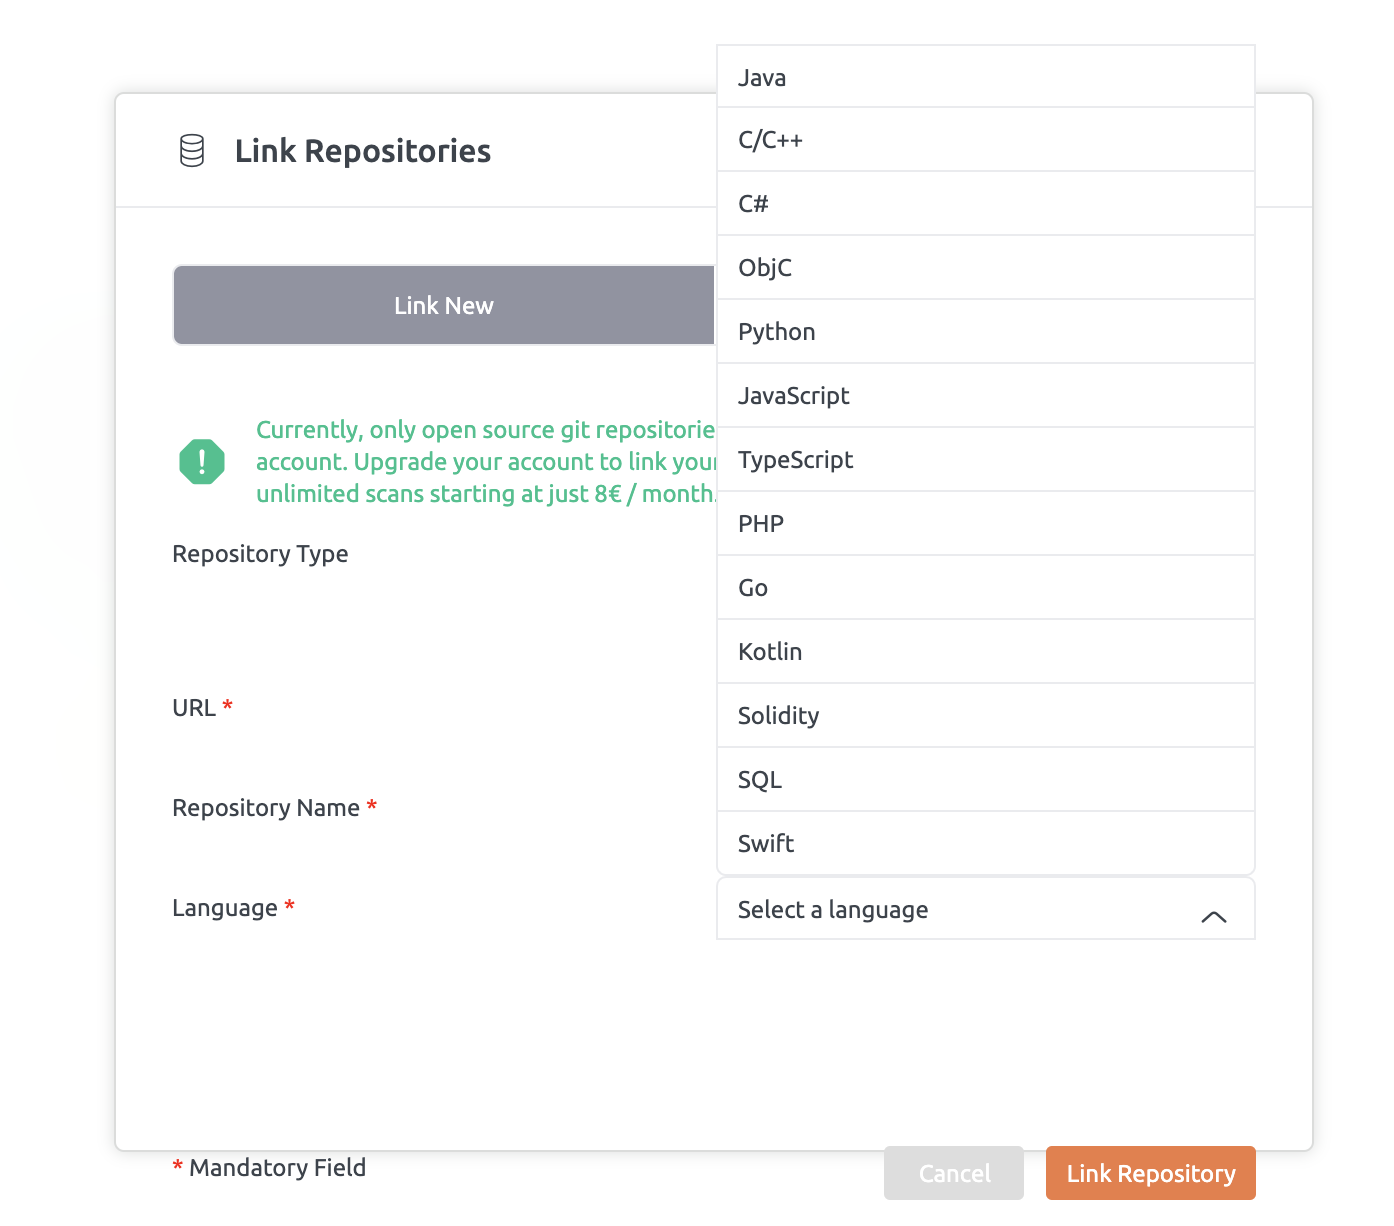
\includegraphics[width=4.5in, height=3in]{negatives.png}
\caption{Programming Languages Availability}
\label{fig:improve}
\end{center}
\end{figure}
\section{Lesson Learned}
I learned about various standards of UX, in depth designing using UCD methodology. It was quite wonderful to have knowledge about the entire design basics and how a little attention could become a big gain for any website. I learnt that it is very important to focus on human needs, extremely important to have iterative approach.\par
It is also important to embrace the change, because human nature is extremely diverse and the most consistent entity in the universe is change. So need to consider ISO standards, work on wireframes and mockups very strongly. Discuss with designers and developers about the design. \par
Along with all this I also got to know about the Embold which is a wonderful tool for various stakeholders in a SDLC. It can be game changer on a healthy scale.

